\chapter{Trazadora. Primera iteración}

Una hoja en blanco es un mundo de posibilidades para algunos, si embargo para mi
es una situación intimidante y abrumadora, la solución es adquirir 
realimentación tan rápido como sea posible.

Un tipo de bala utilizada por los vehículos artillados es la llamada
bala trazadora, tiene la característica de brillar de color rojo cuando es 
detonada y cuando se impacta produce un destello de luz, el objetivo de esta
bala es iluminar la trayectoria del resto de balas cuando son disparadas en 
ráfagas. 

``We use the term tracer bullet development to visually illustrate the need for
immediate feedback under actual conditions with a moving goal.''\cite{pragmatic}

Una implementación no exhaustiva que abarca todas las capas de desarrollo,
el objetivo es el mismo que la trazadora real, iluminar cada una de las capas de
diseño del problema, con suerte podremos ver característica que no 
aparecen a simple vista.

En esta sección expongo la primer iteración correspondiente a una bala
trazadora, recalco que esta iteración busca realimentación del problema
más que satisfacer un requerimiento.

\section{Requerimientos}
\subsection{El movimiento}
Para mi fortuna tengo la asistencia del laboratorio del \emph{Laboratorio de 
Investigación y Desarrollo de Aplicaciones Interactivas para la
Neuro-Rehabilitación} del Instituto de Fisiología Celular de la UNAM, quienes
son expertos y tienen gran experiencia tratando y rehabilitando a este tipo 
de pacientes, la mayor parte del entendimiento y realimentación es gracias a
ellos.

Es aquí donde los objetivos específicos se definen, no antes, cada iteración los
ira refinando. 

Una forma simple de adquirir los requerimientos es por medio de casos de uso,

``A use case is all the ways of using a system to achieve a particular goal for a particular
user.''\cite{ivar}

Es decir los casos de uso son nuestros objetivos.

Un actor es aquel que requiere un caso de uso, para el proyecto un actor
inmediato es el paciente, pues es quien interactúa con el dispositivo de
manera directa y durante la mayor parte del tiempo, sin embargo no es el único,
otro actor muy importante es el operador, usualmente el operador es el médico o
enfermera, él también requiere usar el dispositivo y tiene expectativas en él.
Un tercer actor es el desarrollador, el impone sus caprichos igualmente.
Por ahora estos son los actores identificados, pero no descarto una anexión o 
eliminación en el futuro. Es necesario mencionar que un actor puede no ser 
una persona, puede ser otro sistema o dispositivo.

Los requisitos sintetizados en esta etapa ya se mencionaron en el capitulo 
\ref{objetivos}, se actualizaran al final de la iteración. El primero objetivo/caso
 de uso es

\begin{itemize}
	\item Mover de un punto A a B.
\end{itemize}

Interpretando nuestro objetivo, mover de un punto A a un punto B, es muy amplio,
implementar algo así llevaría mucho tiempo, nuestra prioridad por ahora es obtener
información, así que acotare el objetivo a desplazar el robot hacia adelante nada
más.

\begin{itemize}
	\item Desplazar hacia adelante. 
\end{itemize}
Considero que esta es una buena bala trazadora pues el núcleo del problema es 
mover la posición de un lado a otro.

\subsection{Lenguaje de programación}
Uno de los objetivos es dominar un nuevo lenguaje de programación, 
el lenguaje que lleva la batuta en el mundo del
firmware es \emph{C}, es un lenguaje sencillo, pequeño y con un soporte prácticamente
universal, sin embargo tiene un problema, el tiempo de desarrollo siempre es mayor
que si usáramos lenguajes de más alto nivel. \emph{C++} es un lenguaje que poco a poco 
ha ganado terreno en el software embebido, tiene la ventaja de soportar 
los conceptos de programación orientada a objetos, por otro lado es un 
lenguaje muy complejo, muy grande, difícil de aprender, feo y todos lo odian.

La elección de lenguaje me permito hacerla a capricho, pues me considero un experto
en el lenguaje \emph{C} y uno de mis requisitos es dominar un nuevo lenguaje, que
mejor oportunidad que esta, la elección es C++, aunque igualmente me hubiera 
gustado hacer la implementación en Rust o en Nim, lenguajes modernos que 
pretenden ser no solo una alternativa si no; un reemplazo para C y C++.

\section{Análisis}
Implementaremos el primer requisito.

Hay configuraciones de dispositivos que pudieran realizar esta tarea, 
considero que tomar una de ellas y adaptarla a nuestras necesidades es la opción
correcta. 

\subsection{Selección de robot}
Dentro de los dispositivos disponibles la elección era obvia, un robot, ¿pero  de
que tipo?, estas tres opciones suenan interesantes:
\begin{description}
	\item[Robot antropomorfico] sin duda es el robot más versátil que existe,
		es ampliamente utilizado en la industria manufacturera sobre todo
		en la automotriz, sin embargo tiene una gran desventaja para 
		nuestro propósito, es muy costoso de implementar, principalmente
		por el tipo de actuadores que requiere, esta configuración produce 
		un torque muy grande en su base, lo que deriva en una base de 
		acero y actuadores hidráulicos o neumáticos.
	\item[Robot prismático] Este robot es excelente para movimientos precisos 
		en el plano, es fácil de implementar y soporta cargas muy grandes,
		en un principio esta era una opción muy atractiva, pero tiene un par 
		de desventajas, es relativamente caro y es menos mantenible que 
		la tercera opción.
	\item[Robot móvil] Es la opción que satisface de mejor manera los
		requerimientos, se puede desplazar sobre trayectorias largas, 
		rectas o circulares, es rápido, ligero y de los tres es el más
		barato, no tiene la precisión del robot prismático pero no la 
		requerimos, pocas partes mecánicas y ampliamente documentado. 
		En contraste es más difícil de programar pues requiere más 
		sensores que los anteriores y sus acciones se limitan al plano
		horizontal.
\end{description}

La elección es un robot móvil, ¿con qué características?, con las necessaries, 
las que nos indique el problema para su resolución. Por ahora nos interesa
trasladar el robot hacia adelante, requerimos
\begin{itemize}
	\item Un propulsor.
	\item Una fuente de energía.
	\item Una rutina que haga el trabajo.
	\item Una base que acople todo.
\end{itemize}

\section{Diseño}
Esta sección se trata de pensar, se trata de ver el bosque antes de ver el árbol,
decido dividir el diseño en tres partes, pues evidentemente cada una requiere su 
propio lenguaje y herramientas particulares.
\subsection{Arquitectura electrónica}
El esquemático se muestra a continuación en la figura \ref{fig:Esquemático 1}.

\newschematic{img/esquematico1.pdf}{Esquemático 1}

\subsubsection{Selección de propulsor} 
Lo evidente es que requerimos movimiento, para ello necesitamos
controlar un dispositivo que pueda causarlo,
opciones hay muchas, motores, turbinas, campos de fuerza, la
elección obvia es un motor eléctrico, por el tamaño y el costo principalmente.
¿De que tipo?, por ahora un motor de corriente directa cualquiera nos sirve,
más adelante los requerimientos nos indicaran el adecuado. Decido utilizar
un motor de corriente directa reciclado de una vieja casetera.
Desafortunadamente no cuento con
las características técnicas de este dispositivo,  no tiene marca ni 
leyenda de identificación, procedo a realizar una prueba de rotor libre.

La prueba de rotor libre consiste en medir la corriente que consume el motor 
cuando no tiene carga mecánica, la medición es de tan solo $0.03$ Ampers, con 
una tensión de $9$ volts en sus terminales.

Repito la prueba pero con el robot bloqueado, con la misma tensión, la corriente
sube dramáticamente hasta $500 mA$.

\subsubsection{Selección de dispositivo  programable}
Para controlar un motor hay varias opciones, hablando de dispositivos
programables las opciones se reducen a dos una sbc (computadora
en una sola tarjeta) y microcontroladores, aunque la sbc es mejor en 
prestaciones, es más cara y no es necesaria, existen 
microcontroladores suficientemente poderosos para nuestros objetivos.

De entre los muchos microcontroladores me interesa que tenga documentación 
y soporte, el atmega328p\cite{atmega328p}
del Arduino Uno suele ser la primera opción, pero dada
la complejidad del proyecto me da la sensación de que la memoria programable
puede no ser suficiente, no lo sé, comenzare con este dispositivo y si lo
requiero lo cambio por uno con mayores prestaciones.
\subsubsection{Selección de fuente de poder}
El sistema requiere una fuente de alimentación, baterías son la elección 
adecuada, debido al tamaño y la autonomía, las agregaremos como requisitos y 
más adelante las especificaremos, por ahora cualquier batería con tensión mayor 
a 5 volts basta, me decido por una pila cuadrada de 9 volts.
\subsubsection{Control del motor}
El motor va en un solo sentido, basta con un transistor de propósito general 
que soporte más de 200mA por su colector. Un 2n2222A\cite{2n2222a} es
suficiente.

El transistor se utiliza como switch, se induce una pequeña corriente a través de la
base del transistor, esto provoca que el colector ``se abra'' y pueda conducir una
corriente proporcional a la base, de 100 veces o más para este transistor, 
por ejemplo si inducimos $1mA$ por la base, obtendremos por lo menos $100mA$ por
el colector, este comportamiento nos ayuda mucho, pues el microcontrolador solo 
es capaz de entregar/recibir $20mA$ por cada pin, por su parte el transistor soporta
corrientes continuas de hasta $600mA$.

La forma de inducir la corriente es muy sencilla, se conecta una resistencia 
entre el pin de la base y el pin del microcontrolador como indica el esquemático.
Con ley de Ohm:
\begin{displaymath}
	i_b = \frac{V_{pin} -V_{be}}{R_{b}}
\end{displaymath}
despejando la resistencia 
\begin{displaymath}
	R_b = \frac{V_{pin} -V_{be}}{i_{b}} = \frac{5 - 0.7}{5m}
\end{displaymath}
\begin{displaymath}
	R_b = 860 \Omega
\end{displaymath}
Podemos permitirnos ser conservadores y poner una resistencia de $1000 \Omega$.
\subsection{Arquitectura de software}
Soy electrónico pero soy una persona de software, estás etapas de diseño son muy
satisfactorias para mí. Los planos arquitectónicos de una casa deben verse como
los de una casa y los de una escuela como una escuela, seria absurdo una casa con
fachada de escuela, desafortunadamente la gente de software no alcanza a entender
bien esta idea y programan todo de la misma forma, no es mi caso, mi arquitectura
se verá como un robot móvil.

Me gusta utilizar la arquitectura definida por Robert C. Martin \emph{Clean 
Architecture} \cite{clean_architecture}, es un modelo basado en 
capas, donde la capa más 
profunda es constituida por las llamadas entidades criticas, las capas intermedias
por las reglas de negocio y las capas exteriores las componen los detalles.
\begin{description}
	\item[Entidades criticas] Son estructuras de datos u objetos que solo 
		contiene datos y no funcionalidad. Tienen una característica muy
		descriptiva, lejos de ser abstractas son muy concretas y cambian
		muy poco, es una buena idea depender de entes concretos, es decir
		todos las entidades deben depender de las entidades criticas, queda
		prohibido que las entidades criticas dependendan de los detalles. 
	\item[Reglas de negocio] Mejor conocidas como business rules, son 
		funcionalidades que modifican y/o acceden a las entidades criticas
		para satisfacer los requerimientos. Nuestro robot requiere avanzar,
		usaremos software para controlar el avance, sin embargo el software
		no es necesario, bien podríamos empujar el robot, o hacer que un
		caballo lo jale, hay muchas formas de hacerlo avanzar, a eso me 
		refiero con regla de negocio, a un procedimiento que realiza el 
		dispositivo no importando si esta automatizado por software o no.
	\item[Detalles] Todo aquello fuera del negocio, generalmente periféricos.
		Los detalles no tienen que ver con el negocio, son simples 
		elecciones a capricho o a conveniencia, por ejemplo, el tipo de 
		motor, al robot no le interesa que tipo de motor hay, tan solo
		le interesa que al enviarle un comando el motor giré y provoque el
		avance. 
\end{description}

Requerimos mover el robot, a continuación enumero el bosque:
\begin{enumerate}
		
	\item	Por ahora solo se requiere ir hacia adelante, un solo pin de propósito
		general basta para lograrlo.

	\item No hay requerimientos de distancia, así que un temporizador sera 
		suficiente.

	\item Un pulsador conectado a un pin para iniciar la secuencia.
\end{enumerate}

Por ahora pienso que es suficiente, el diagrama de bloques de la arquitectura 
se muestra en la figura\ref{fig:arquitecturaSoftware1}.

\begin{figure}[hbtp]
	\centering
	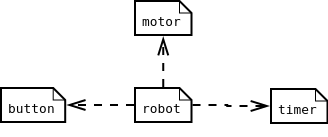
\includegraphics[scale=0.5]{img/arquitecturaSoftware1}
	\caption{Arquitectura de software 1.1}
	\label{fig:arquitecturaSoftware1}
\end{figure}

Robot es una entidad que depende de timer, motor y button, acabo de mencionar 
que esta prohibido que capas centrales dependan de capas externas, la forma de 
arreglan esto es utilizar interfaces. 

Una interfaz es una clase que no tiene parámetros, solo métodos, y los métodos son del tipo
virtual\footnote{Un método virtual tiene la características de poder ser 
redefinido por las clases heredadas}.

No se pueden crear instancias/objetos de interfaces, ¿entonces para que y como se
usan?, la respuesta no es trivial, su principal objetivo es desacoplar módulos/clases,
sin embargo también sirven para extender clases y también es posible revertir 
dependencias. Dada una interfaz, por ejemplo Motor, se pueden implementar nuevas
clases derivadas de motor, MotorDC, MotorAC, etc, al ser clases derivadas siguen
siendo Motor y contienen la misma funcionalidad, el como lo logran es un detalle, 
pero su \emph{cara} hacia el mundo es la misma. Dicho esto, se propone la arquitectura 
de la figura \ref{fig:arquitecturaSoftware1.2}.
\begin{figure}[hbtp]
	\centering
	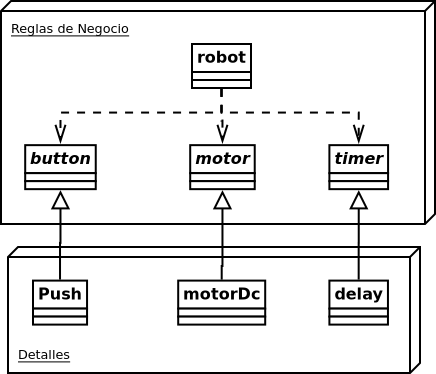
\includegraphics[scale=0.5]{img/arquitecturaSoftware1.2}
	\caption{Arquitectura de software 1.2}
	\label{fig:arquitecturaSoftware1.2}
\end{figure}
Ahora robot ya no depende de los detalles, los detalles dependen de las reglas de
negocio.

\subsection{Arquitectura mecánica}
Por último pero no al final, la arquitectura mecánica, a diferencia de la 
electrónica y la programación la parte mecánica tiene un contacto directo con el
paciente, es necesario poner suficiente esfuerzo pues de ella dependerá en gran
proporción la satisfacción del paciente.

El diagrama es sencillo en esta etapa, solo requerimos una superficie que soporte
todos los componentes, propongo el esquema mostrado en la figura 
\ref{fig:Plano 1},
\newdraw{img/plano1.pdf}{Plano 1}
Consiste de una base circular soportada por 4 pequeños postes y exactamente a la
mitad un motor, por supuesto la mayor parte de esto cambiara con conforme el 
desarrollo avance.
\section{Implementación}
Las tres partes pueden implementarse en forma individual y paralela, al final se
hará una etapa de integración.\footnote{En esta etapa es donde se diferencian los
hombres de los niños}. Por simple gusto implemento primero la parte mecánica.
\subsection{Implementación mecánica}
Cualquier material nos sirve para hacer la base, me decido por utilizar cartón,
es fácil de manipular y barato, para los soportes utilizo lapices, la llanta es
reciclada de un juguete y el motor también es reciclado.

El resultado es un juguete muy feo, pero me da las sensaciones que estaba 
buscando figura \ref{fig:robot1}.
\begin{figure}[hbtp]
	\centering
	\makebox[0.9\textwidth][c]{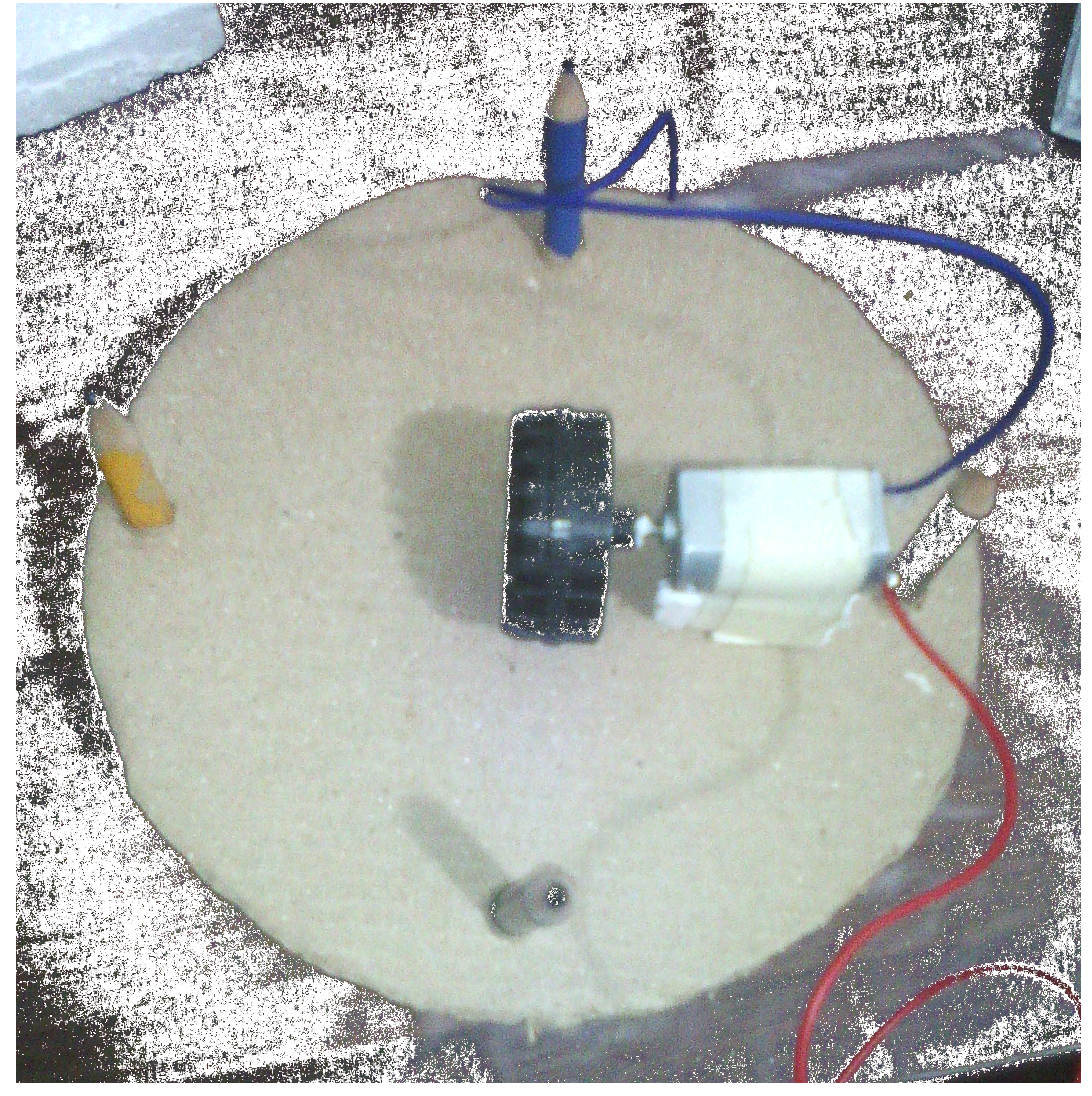
\includegraphics[angle=90, width=\textwidth]{img/robot1}}
	\caption{Robot 1}
	\label{fig:robot1}
\end{figure}

\subsection{Implementación electrónica}
Para facilitar la implementación utilizo un Arduino nano, tiene incorporado un 
regulador de tensión de $5V$, no tendré que preocuparme por regular por ahora, 
tan solo se realiza el cableado indicado en el esquemático en una tablilla de
prototipos.
\subsection{Implementación del programa}
La implementación mecánica y eléctrica fue sencilla, pero la programación requiere
más tiempo y cuidado, sobre todo la primera vez.

Es muy complicado explicar el proceso de programación, la forma correcta sería 
colocar el código y su evolución con cada una de las decisiones de diseño que
tomamos, pero para un programa de 10 lineas, tendría que mostrar unas 20 versiones,
pasando por cada una de las pruebas unitarias. Prefiero mostrar únicamente las 
partes que considero relevantes.

\subsubsection{Robot}
Aprovechando los conceptos de modularidad y programación orientada a objetos
creamos una clase robot, por agregación tiene tres apuntadores, son los objetos 
que utiliza el robot, su constructor\footnote{El constructor de una clase es un
método que se ejecuta automáticamente al crear una instancia de la clase} y por
supuesto la acción que nos interesa, moverse hacia adelante. Los $\#include$
contienen la declaración de las interfaces.
\begin{minted}[linenos]{C++}
#ifndef ROBOT_H
#define ROBOT_H

#include "motor.h"
#include "timer.h"
#include "button.h"

class Robot{
	private:
		Button * button_;
		Motor * motor_;
		Timer * timer_;
	public:
		Robot(Motor *, Timer *, Button *);
		void moveFordward(void);
};
#endif // ROBOT_H
\end{minted}
La clase es simple, el constructor recibe apuntadores a instancias de las clases
Motor, Timer y Button,\footnote{Realmente recibe apuntadores a instancias 
derivadas de estas.} y las asigna a los apuntadores dentro de la clase robot.
Veamos la implementación de los dos métodos.
\begin{minted}[linenos]{c++}
#include "robot.h"

Robot::Robot(Motor * motor, Timer * timer, Button * button):
	motor_{motor}, timer_{timer}, button_{button}
{
}
void Robot::moveFordward(void)
{
	if(button_->pushed()){
		motor_->on();
		timer_->enable();
		while(timer_->getTime() <= 1000);
		motor_->off();
	}
}
\end{minted}
El método constructor muestra un concepto muy interesante, llamado dependency 
injection, 
dentro del diseño de software la inyección de dependencias es una forma de lograr
desacoplar al módulo de sus dependencias, nosotros requerimos un motor, pero al
solo pasar un apuntador o referencia, nos liberamos de conocer los detalles de 
su implementación, el robot solo sabe que existe un motor y que lo puede encender o
apagar, pero no tiene idea de como esta conectado, de que tipo es, de corriente directa o
alterna, tamaño o potencia, etc, lo mismo para el temporizador y botón.

Inicializados los apuntadores, los usamos para acceder a los métodos y creamos una 
sencilla rutina, se explica por si sola, si el botón está presionado, enciende el 
motor por un segundo.
\subsubsection{Motor}
¿Y como se implementa el motor con interfaces?,
\begin{minted}[linenos]{C++}
#ifndef MOTOR_H
#define MOTOR_H
class Motor{
	public: 
		virtual void on(void) = 0;
		virtual void off(void) = 0;
};
#endif// MOTOR_H
\end{minted}

La interfaz motor muestra dos métodos virtuales con una sintaxis un poco extraña,
el termino $= 0$, es la forma que tiene \emph{C++} de indicar que una clase es una
interfaz, la palabra $virtual$, indican que las clases que hereden de ella pueden
sobreescribir el método.

Ahora describirnos una clase con un motor particular de DC,
\begin{minted}[linenos]{C++}
#ifndef MOTORDC_H
#define MOTORDC_H

#include "motor.h"

class MotorDc : public Motor{
	public:
		MotorDc(short const pin);
		virtual void on(void) override;
		virtual void off(void) override;
};
#endif// MOTORDC_H
\end{minted}

Lo importante de esta clase es que hereda de la interfaz $Motor$ y que $override$
obliga a definir los  métodos virtuales, 
independientemente del tipo de motor que se defina, seguirá 
siendo del tipo $Motor$, pues heredan de él y seguirán teniendo que 
implementar ambas funciones $on$ y $off$. La implementación es:

\begin{minted}[linenos]{C++}
#include "motorDc.h"
#include <avr/io.h>

MotorDc::MotorDc(short const pin)
{
	DDRD |= 1<<PD3;
}
void MotorDc::on(void)
{
	PORTD |= 1<<PD3;
}
void MotorDc::off(void)
{
	PORTD &= ~(1<<PD3);
}
\end{minted}

Programar un microcontrolador puede resumirse a modificar sus registros\footnote{
Un registro es una locación de memoria en el microcontrolador, modificar los 
registros implica modificar el comportamiento del hardware}, 

Para implementar el motor modificamos dos registros, \textbf{DDRD} y \textbf{PORTD},
el primero Data direction register, nos permite configurar a el pin como entrada
o salida, el método constructor configura al pin \textbf{PD3} como salida, el 
segundo registro nos permite indicar el nivel lógico, bajo o alto, 0 o 5 volts, 
respectivamente. Las funciones on y off modifican este registro, escribiendo
nivel alto y bajo.

Para acceder a los registros es necesario incluir la biblioteca $avr$ adecuada, 
es este caso $io.h$.
\subsubsection{Botón}
El módulo Button es igual a Motor, salvo que el pin \textbf{PD2}, se configura 
como entrada en \textbf{DDRD}, cuando un pin se elije como entrada, se obtiene 
una impedancia muy grande en el mismo adicionalmente \textbf{PORTD}
tiene un comportamiento diferente, escribir un uno lógico implica conectar una
resistencia de Pull Up\footnote{Una resistencia conectada a Vcc}, activar
esta resistencia tiene una gran utilidad, pues sin ella la alta impedancia en el 
pin provoca una gran sensibilidad al ruido electromagnético. La interfaz es la
siguiente
\begin{minted}[linenos]{C++}
#ifndef BUTTON_H
#define BUTTON_H
class Button{
	public:
		virtual bool pushed(void) = 0;
};
#endif// BUTTON_H
\end{minted}
Tan solo cuenta con un método virtual que nos indica se el botón esta pulsado o no.
La definición de un botón particular es:
\begin{minted}[linenos]{C++}
#ifndef PUSH_H
#define PUSH_H

#include "button.h"

class Push : public Button{
	public:
		Push(short const pin);
		virtual bool pushed(void) override;
};
#endif// PUSH_H
\end{minted}
y la implementación:
\begin{minted}[linenos]{C++}
#include "push.h"
#include <avr/io.h>

Push::Push(short const pin)
{
	DDRD &= ~(1<<PD2);
	PORTD |= 1<<PD2;
}

bool Push::pushed(void)
{
	if((PIND&(1<<PD2)) == 0)
		return true;
	else
		return false;
}
\end{minted}
Para leer el estado de un pin se consulta el registro \textbf{PIND}.
\subsubsection{Timer}
Timer es prácticamente idéntica en cuanto a la interfaz y descripción, por lo 
que solo muestro la implementación.
\begin{minted}[linenos]{C++}
#include "timer_delay.h"
#include <util/delay.h>

void Timer_delay::enable(void)
{
}
unsigned long Timer_delay::getTime(void)
{
	_delay_ms(1000);
	return 1000;
}
\end{minted}
Utilizo la función $\_delay\_ms$ provista por $delay.h$, para crear una pequeña
pausa y después retorno $1000$,
es un poco hardcoded,\footnote{Hecho a mano, connotación negativa por ser una mala
práctica} pero funciona y es probable que esto se borre en la próxima iteración. 
\subsubsection{Main}
Finalmente enlazamos los módulos en la función main,
\begin{minted}[linenos]{C++}
#include "robot.h"
#include "timer.h"
#include "button.h"
#include "motor.h"
#include "motorDc.h"
#include "timer_delay.h"
#include "push.h"


int main(void)
{
	MotorDC motor(1);
	Timer_delay timer;
	Push push(2);
	Robot robot(&motor,&timer, &push);

	while(1){
		robot.moveFordward();
	}

	return 0;
}
\end{minted}
Creamos los objetos de las instancias adecuadas y pasamos las direcciones al 
robot. El número que pasamos al motor y al botón push al construirlos indica el
pin al que están conectados, en este momento no están implementados, no seguí mi
propia regla y me adelanté, añadí algo que aun no necesito, seré más cuidadoso en
el futuro. 
\section{Pruebas}
Las pruebas son someras para este caso, tan solo nos interesa que el robot se 
mueva hacia adelante, no importa la velocidad ni la distancia, ni si quiera que lo
haga en línea recta o de manera uniforme.

Las observaciones son las siguientes:
\begin{itemize}
	\item El robot se mueve hacia adelante.
	\item El motor gira muy rápido y patina.
	\item La trayectoria es corta y no es rectilínea. 
	\item Soporta poca carga.
	\item La carga eléctrica sube dramáticamente con carga mecánica. 
	\item Las dimensiones de la llanta limitan la dimensión del motor.
	\item La nueva prioridad es añadir otro motor y realizar nuevamente el objetivo
		de mover hacia adelante.
\end{itemize}

Parece ser que perdí el tiempo, aunque el objetivo se logró, se encontraron muchas 
sensaciones negativas, entonces ¿no valió la pena la bala trazadora?, pienso que 
valió totalmente la pena, el tiempo de implementación fue relativamente corto,
pero lo más importante fue la información que se obtuvo, ahora ya no tengo una
hoja en blanco, si no una hoja de ruta, las sensaciones se reflejan en la refinación
de objetivos.

\section{Objetivos refinados}
\begin{itemize}
	\item Para el paciente.
		\begin{enumerate}
			\item Mover el robot de un punto A a B.
				\begin{itemize}
					\item Mover hacia adelante.
					\item Mover hacia atrás.
					\item Mover hacia adelante/atrás, en línea
						recta.
					\item Mover hacia adelante una x distancia.
					\item Mover hacia atrás una x distancia.
					\item Mover hacia adelante/atrás y girar hacia
						la derecha/izquierda.
					\item Girar x grados.
					\item Mover sobre una trayectoria curva.
				\end{itemize}
			\item Potencia suficiente para soportar la carga.
				\begin{itemize}
					\item Suministro de corriente adecuado.
					\item Tamaño y materiales de la llanta.
					\item Motores con el tamaño y torque adecuado.
					\item Acoplamiento con la base.
				\end{itemize}
			\item Movimiento save.
				\begin{itemize}
					\item Control de la velocidad.
					\item Control de la aceleración.
					\item Control diferenciado de ambos motores.
					\item Generación y seguimiento de trayectorias.
				\end{itemize}
			\item Rotación libre.
				\begin{itemize}
					\item Basé rígida y pesada.
					\item Acoplamiento encima la base.
				\end{itemize}
		\end{enumerate}
	\item Para el médico.
		\begin{enumerate}
			\item Interfaz de trayectorias.
		\end{enumerate}
	\item Para el desarrollador.
		\begin{enumerate}
			\item Dominar un nuevo lenguaje de programación.
			\item Metodologías RUP y XP.
		\end{enumerate}
\end{itemize}
